% !TEX TS-program = pdflatex   
\documentclass[runningheads,12pt]{article} 
\usepackage{graphicx}
\usepackage{color,url}
\usepackage{mdframed}%put frame around text or a table
\usepackage{pdfpages}% Import pdf
\usepackage{soul}% Highlight

\usepackage{sty/bsymb} %% Event-B symbols
\usepackage{sty/eventB} %% REQ and ENV
%\usepackage{sty/b2latex}% Importing from Rodin
\usepackage{sty/calculation} % Calculational proofs
\newcommand{\term}[1]{\textit{#1}}

\usepackage{fancyhdr,lastpage}
\lhead{\rm EECS3342 --- Report Template}
\rhead {\rm Page \thepage~of \pageref{LastPage}}
\lfoot{}\cfoot{}\rfoot{}
\pagestyle{fancy}

\begin{document}

\title{EECS3342 --- Report Template\\
Put your report name here}


\maketitle


\noindent Submit only under one Prism Login.\\
Teams may have a maximum of two members.\\
Your signature affirms that this is solely your work.

\begin{table}[h]
\begin{tabular}{l|l|l|l|l|}
\cline{2-5}
& First Name  & Last  Name & Prism Login & Signature \\ \hline
\multicolumn{1}{|l|}{Student1}                                                            
&                &                    &                 &                      \\ \hline
\multicolumn{1}{|l|}{Student2}                                                            
&            &            &             &           \\ \hline
\multicolumn{1}{|l|}{\begin{tabular}[c]{@{}l@{}}Prism Login\\ of submission\end{tabular}} 
&             &            &             &           \\ \hline
\end{tabular}
\end{table}

\hl{Prepare the documentation for the assignment and the project professionally.}

Rodin produces Latex documentation, so this is a good method for documenting your specifications and refinements. See \url{https://wiki.eecs.yorku.ca/project/sel-students/p:tutorials:latex:start} for an introduction to Latex. Login at the bottom with your Prism login.

\newpage
\tableofcontents
\listoffigures
%\listoftables
\newpage

%%%%%%%%%%%%%%%%%%%%%%%%%%%%%%%%%%%%%%%%%%%%
\section{Initial model, first and second refinement}

The initial model, and first and second refinement are as in the textbook. The initial model is shown in Fig.~\ref{fig:m0}.

An image of all the proofs successfully discharged for the initial model is provided below:

\includegraphics[width=.5\textwidth]{images/m0-proof.png}


\bigskip
\hl{Student: the above is just to help you structure your document in Latex. You must document the complete specification and refinement including contexts, machines and any E and R descriptions. Explain in the text the idea behind each refinement}

%%%%%%%%%%%%%%%%%%%%%%%%%%%%%%%%%%%%%%%%%%%%
%Example of importing PDF pages generated from the Rodin Plugin
% Do clearpage so that successive pdf pages are not interrupted.
\clearpage
\section{Importing PDF pages}
This is how you import PDF pages (perhaps generated by the Latex Plugin of Rodin). PDF pages start from the next page



\includepdf[pages=-]{pdf/c0.pdf}
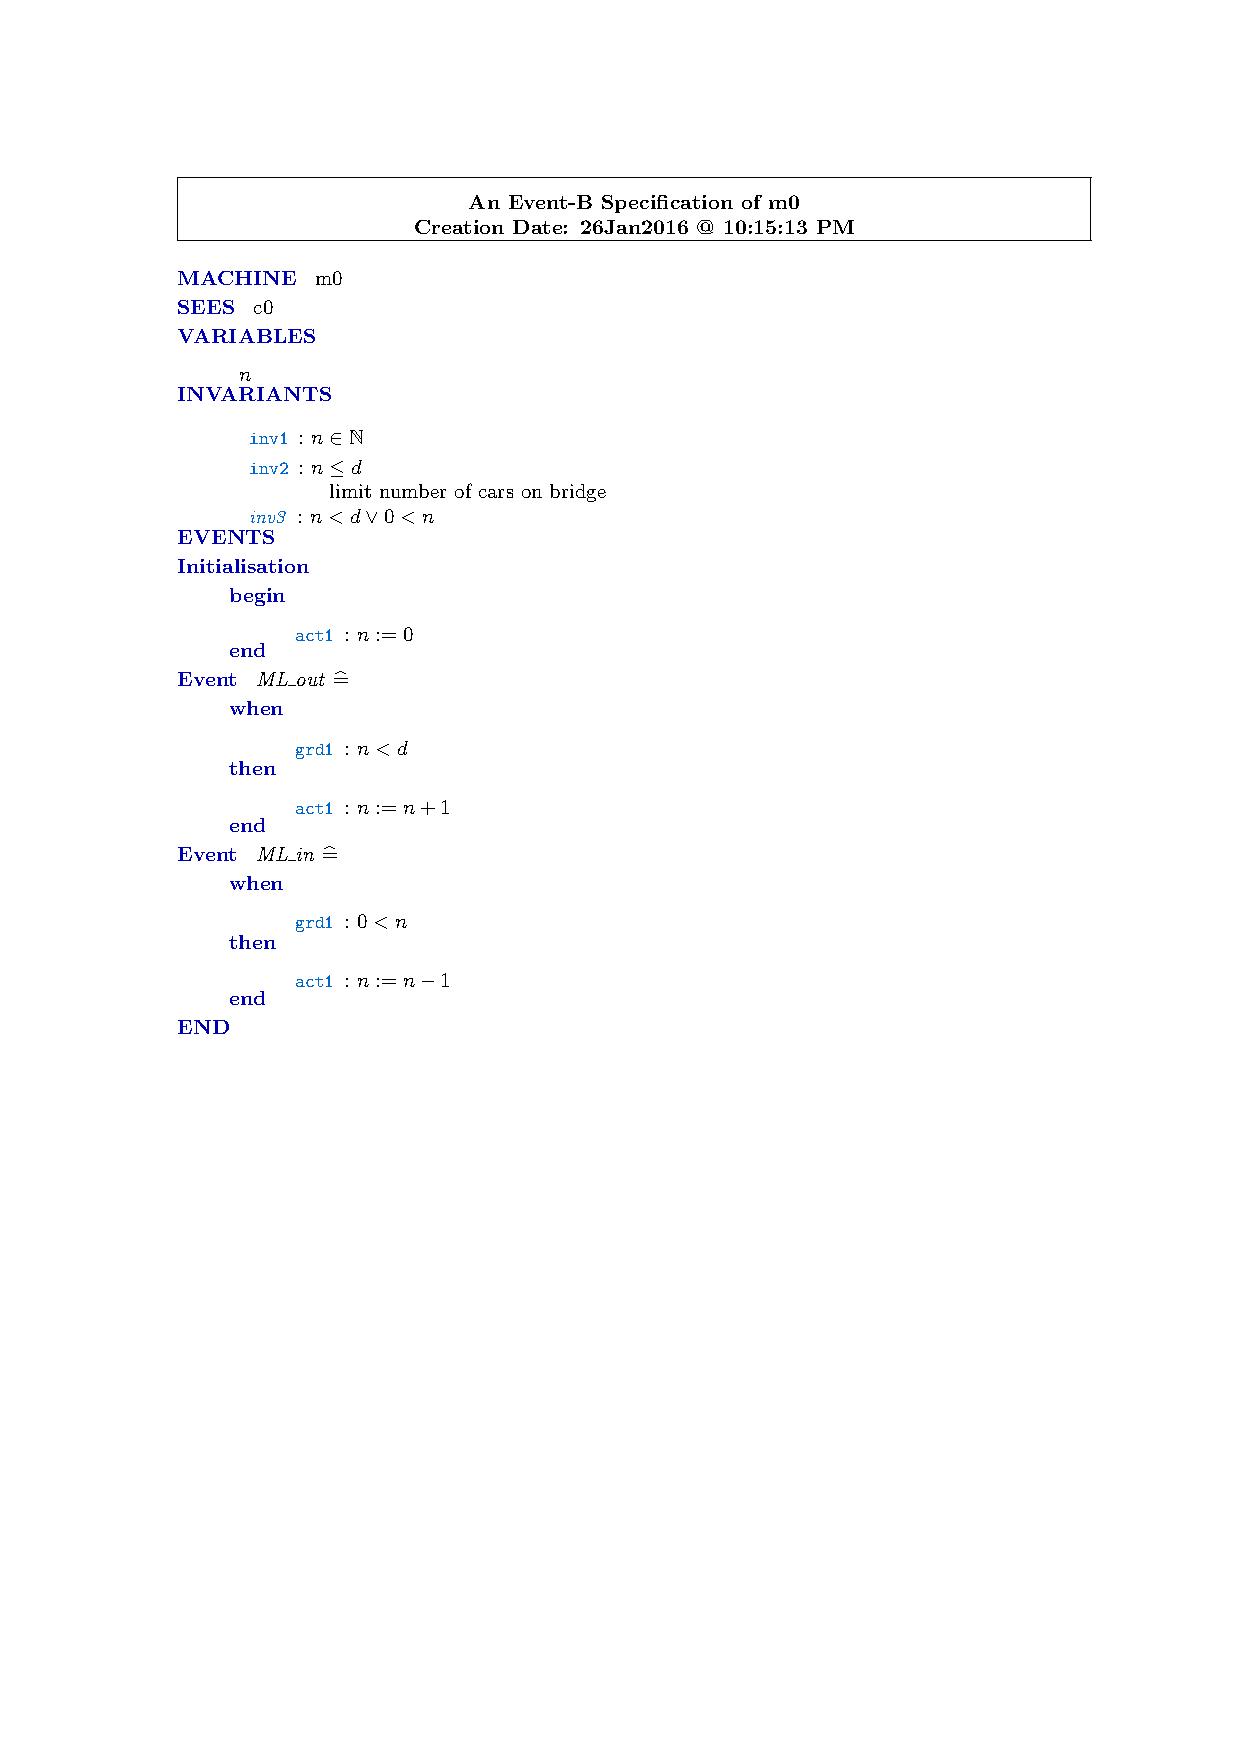
\includepdf[pages=-]{pdf/m0_and_m1.pdf}
\clearpage
%%%%%%%%%%%%%%%%%%%%%%%%%%%%%%%%%%%%%%%%%%%%
\section{Third refinement to complete the implementation of the final event}


%%%%%%%%%%%%%%%%%%%%%%%%%%%%%%%%%%%%%%%%%%%%



\end{document}